
\section{Bayesian Image Reconstruction}


\newcommand{\mrirecon}{
\begin{tikzpicture}[scale=0.75, every node/.style={scale=0.75}]

\def\rightimgX{4.2}

%Top left
% \filldraw[fill=gray!50!white, draw=black, label={Latent}] (-2,2.5) rectangle (-1.5,4.5);
% \node (rng_text) at (-1.75,4.75) {\footnotesize{Latent}};
% \node (rng_text) at (-1.75,3.5) {$w$};

%top image center
\node (cxr_img) at (\rightimgX, 3.5) {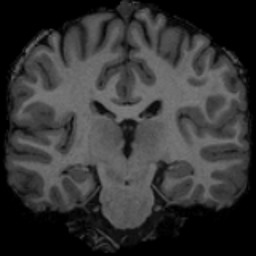
\includegraphics[width=2cm]{\diagfld/brain_clean}};
% \node (cxr_text) at (1,4.75) {\footnotesize{High Res.}};

%top image right
\node (blur_img) at (1, 3.5) {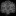
\includegraphics[width=2cm]{\diagfld/brain_target}};
% \node (blur_text) at (\rightimgX,4.75) {\footnotesize{Low Res.}};

% \node (rng_top_out) at (-1.5,3.5) {};
% \node (center_img_left_in) at (0, 3.5) {};

% \draw[->, thick]
% (rng_top_out)
% to
% (center_img_left_in) ;

\node (left_img_top_out) at (2,3.5) {};
\node (right_img_top_in) at (\rightimgX - 1, 3.5) {};

\draw[->, thick]
(left_img_top_out)
to
(right_img_top_in) ;

% \node (left_img_top_in) at (2,2.5) {};
% \node (right_img_top_out) at (\rightimgX - 1, 2.5) {};

% \node (left_img_bot_out) at (0,2.5) {};
% \node (rng_bot_out) at (-1.5, 2.5) {};


% \node (rng_text) at (-0.75,3.75) {$G(w)$};
% \node (rng_text) at (-0.75,3.25) {\fstikz{Image}};
% \node (rng_text) at (-0.75,3) {\fstikz{Generation}};

% \node (rng_text) at (2.75,3.75) {$f_1$};
% \node (rng_text) at (2.75,3.25) {\fstikz{Known}};
% \node (rng_text) at (2.75,3) {\fstikz{Corruption}};

\end{tikzpicture}
}


\newcommand{\brgmfull}{
\begin{tikzpicture}[scale=0.75, every node/.style={scale=0.75}]

\def\rightimgX{4.2}

%Top left
% \filldraw[fill=gray!50!white, draw=black, label={Latent}] (-2,2.5) rectangle (-1.5,4.5);
% \node (rng_text) at (-1.75,4.75) {\footnotesize{Latent}};
% \node (rng_text) at (-1.75,3.5) {$w$};

%top image center
\node (cxr_img) at (\rightimgX, 3.5) {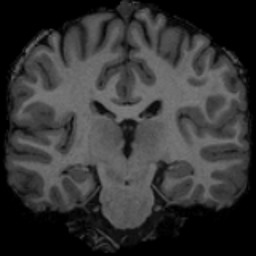
\includegraphics[width=2cm]{\diagfld/brain_clean}};
% \node (cxr_text) at (1,4.75) {\footnotesize{High Res.}};

%top image right
\node (blur_img) at (1, 3.5) {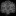
\includegraphics[width=2cm]{\diagfld/brain_target}};
% \node (blur_text) at (\rightimgX,4.75) {\footnotesize{Low Res.}};

% \node (rng_top_out) at (-1.5,3.5) {};
% \node (center_img_left_in) at (0, 3.5) {};

% \draw[->, thick]
% (rng_top_out)
% to
% (center_img_left_in) ;

\node (left_img_top_out) at (2,3.5) {};
\node (right_img_top_in) at (\rightimgX - 1, 3.5) {};

\draw[->, thick]
(left_img_top_out)
to
(right_img_top_in) ;

 \node (left_img_top_in) at (2,2.5) {};
 \node (right_img_top_out) at (\rightimgX - 1, 2.5) {};

% \node (left_img_bot_out) at (0,2.5) {};
 \node (rng_bot_out) at (-1.5, 2.5) {};


 \node (rng_text) at (-0.75,3.75) {$G(w)$};
 \node (rng_text) at (-0.75,3.25) {\fstikz{Image}};
 \node (rng_text) at (-0.75,3) {\fstikz{Generation}};

% \node (rng_text) at (2.75,3.75) {$f_1$};
 \node (rng_text) at (2.75,3.25) {\fstikz{Known}};
 \node (rng_text) at (2.75,3) {\fstikz{Corruption}};

\end{tikzpicture}
}

\begin{frame}{Aim: image reconstruction using *pre-trained* generator models}

\begin{columns}
 \begin{column}{0.5\textwidth}
  
  \begin{itemize}
   \item Adapt the state-of-the-art StyleGAN2 for medical image reconstruction

%    \vspace{2em}
   
%    \item Vision: bring this technology to medicine
  \end{itemize}
  
 \vspace{1em}
 
%   \begin{column}{0.5\textwidth}
%   \centering
% %   MRI generation\\
% %   \incw{\diagfld/brain_clean}{0.4}
% 
%   \end{column}
  \begin{column}{\textwidth}
  \centering
  MRI reconstruction\\
  \mrirecon
  
  \end{column}
  
 \end{column} 
 
 \begin{column}{0.5\textwidth}
 \centering
 StyleGAN2 (Karras et al, 2019)
 \incw{stylegan}{0.8} 
 \end{column}

\end{columns}



\end{frame}

\begin{frame}{Current image reconstruction methods have several limitations}


\begin{columns}
 \begin{column}{0.5\textwidth}

 \begin{itemize}
 \item Require large computational resources and data
 
 \vt
 
 \item Are specific to particular corruption tasks
 
 \vt 
 
 \item Cannot deal with distribution shifts:
 \begin{itemize}
   \item in inputs: e.g. older populations
   \item in corruption type: e.g. change in blur kernel
 \end{itemize}
 
  
 \end{itemize}

 \end{column}

 \begin{column}{0.5\textwidth}
  \centering
%\incw{task-specific}{0.8}
 \brgmprev  
  
 \end{column}
\end{columns} 

 
\end{frame}



\begin{frame}{Limitation 1: State-of-the-art DL methods have large computational requirements}

\begin{itemize}
\item Requirements = Computation Time + Advanced Hardware + Large Datasets

\vo 

\item Most computation now runs on clouds\\ 
%  \begin{itemize}
%  \item Large computational resources
%  \item Large datasets
%  \item Long time to converge
% \end{itemize}

 \incw{datacenter}{0.5}

\vo

 \item Currently few labs/companies have the resources to train state-of-the-art models
 \begin{itemize}
  \item StyleGAN2: 9 days on 4 GPUs
  \item GPT-3: 355 years on single GPU
 \end{itemize}

 
\vo


\vo
 \item Solutions moving forward:
 \begin{itemize}
\item Adapting previously-trained models
\item Combine smaller models into larger ones
\end{itemize}
\end{itemize}

 
\end{frame}

\begin{frame}{Limitation 2: Distribution shifts require model re-training}


\begin{itemize}
 \item Distribution shifts happen all the time:
 \begin{itemize}
 \item Changes in hospital scanners, protocols, software upgrades
 \item Can be continuous: population getting older due to better healthcare
\end{itemize}

\vt
 \item Shifts can result in combinatorial effects in number of re-training instances!

\vt
 
 \item Compositionality is one potential solution
 
\end{itemize}
% \vspace{1em}

\begin{center}
\incw{compositionality}{1}
\end{center}
 
\end{frame}


\begin{frame}{Limitation 3: Models are anti-causal}


\begin{itemize}
 \item Existing model don't follow the data-generation process
\begin{itemize}
   \item Discriminative modelling easier than generative
\end{itemize}

 \vo
 
  
 \vo 
 
 \item Causal modelling is the \textbf{right solution} to deal with distribution shifts
 
 \vo
 
%  \begin{itemize}
%  \item Both for inputs and intermediary variables
% \end{itemize}
\end{itemize}


\begin{center}
\incw{causality}{0.8}
\end{center}
 
\end{frame}


\begin{frame}{Method: We perform image reconstruction by combining two models\\
% \begin{itemize}
\ \ \ \ \ \  1. a pre-trained generator G (StyleGAN2)\\
\ \ \ \ \ \  2. a known forward corruption model $f_1$
% \end{itemize}
}



\begin{columns}[t]
 \begin{column}{0.6\textwidth}
\centering
 
\begin{overprint}
 %\onslide<1> \incw{brgm_diagram_loss}{1}
 %\onslide<2-> \incw{brgm_diagram_all}{1}
 
 \onslide<1> \brgmoursshortloss 
 \onslide<2-> \brgmours

\end{overprint} 
 \onslide<3> Ours (Marinescu et al, arXiv, 2020)
 \end{column}

 \begin{column}{0.3\textwidth}
  \centering

 %\onslide<3> \incw{task-specific}{1}
 \onslide<3> \brgmprev
 \onslide<3> Previous

 
 \end{column}
\end{columns} 
 


 
\end{frame}

\newcommand{\ci}[1]{\circ{#1}}
\newcommand{\wplus}{$\mathcal{W}^{+}$ }
\newcommand{\loss}{\mathcal{L}}

\newcommand{\bit}[1]{\begin{itemize} 
\item #1
\end{itemize}}

\begin{frame}{Reconstructed image is given by computing the Bayesian maximum a-posteriori (MAP) estimate\\
}



\begin{itemize}
 \item We optimise:
$$ w^* = \argmax_w p(w)p(I|w)$$

\item For uninformative prior $p(w)$ and Gaussian noise model (pixelwise independent), we get:

$$ w^* = \argmin_w || I - f \circ G (w) ||_2^2$$

\item This can be optimised with SGD

\item Once we get $w^*$, the the reconstructed image is $G(w^*)$

\end{itemize}

\begin{center}
\vt
%\incw{brgm_diagram_loss}{0.6}
\brgmoursshortloss
\end{center}
 
\end{frame}
% 

\newcommand{\txc}[1]{\mathbin{\textcolor{red}{#1}}}
\newcommand{\szb}{0.8}
\begin{frame}{Good reconstructions require further modifications}

\begin{columns}

\begin{column}{0.5\textwidth}
\begin{itemize}
  \item We started from the original StyleGAN2 inversion
 
 \vo
 
 \onslide<2-> \item Yet the reconstruction was not good $\to$ required several changes
\begin{overprint}
\onslide<3> \bit{remove noise layers}
\onslide<4> \bit{optimize latents at all resolutions}
\onslide<5> \bit{add pixelwise loss}
\onslide<6> \bit{gaussian prior on latents}
\onslide<7> \bit{force latents to be colinear}
\onslide<8> \bit{Analytically expressed the full likelihood (Marinescu et al, 2021)}
\end{overprint}


%  \vo
%  
%  \onslide<2-> \item We reached suitable solutions only after several changes 
%  \item Finall posterior likelihood function was:
 
% \begin{equation}
% \begin{aligned}
% \label{bfinal}
% & w^* = \argmin_w \underbrace{\sum_i \left(\frac{w_i-\mu}{\sigma_i}\right)^2}_\text{prior on $w$} - 2\kappa \underbrace{\sum_{i,j} \frac{w_iw_j^T}{|w_i| |w_j|}}_\text{colinearity} \\
% & + \sigma_{pixel}^{-2} \underbrace{\norm{I - f \ci G(w)}_2^2}_\text{pixelwise loss} + \sigma_{percept}^{-2} \underbrace{\norm{I - \phi \ci f \ci G(w)}_2^2}_\text{perceptual loss} \\
% \end{aligned}
% \end{equation}
 
\end{itemize}
\end{column}
\begin{column}{0.5\textwidth}

% % \begin{overprint}
% \begin{overlayarea}{0.5\textwidth}{0.3\textheight}
% \only<1>{ \begin{equation} w^* = \argmin_w || I - f \circ G (w) ||_2^2 \end{equation} }
% \only<2>{ \begin{equation} w^* = \argmin_w **|| I - f \circ G (w) ||_2^2 \end{equation} }
% \end{overlayarea}
% % \end{overprint}

\begin{overprint}
\onslide<0-2> \begin{equation*} w^*, \txc{\eta^*} = \argmin_{w,\txc{\eta}} || \phi(I) - \phi \circ f \circ G (w, \txc{\eta}) ||_2^2 \end{equation*}
\onslide<3> \begin{equation*} w^* = \argmin_{w} || \phi(I) - \phi \circ f \circ G (w) ||_2^2 \end{equation*}
\onslide<4> $$\txc{\textbf{w} = w_1,..,w_L}$$ \begin{equation*} \txc{\textbf{w}^*} = \argmin_{\txc{\textbf{w}}} || \phi(I) - \phi \circ f \circ G (\txc{\textbf{w}}) ||_2^2 \end{equation*}
\onslide<5> \begin{equation*} \textbf{w}^* = \argmin_{\textbf{w}} || \phi(I) - \phi \circ f \circ G (\textbf{w}) ||_2^2 \txc{+ || I - f \circ G (\textbf{w}) ||_2^2} \end{equation*}
\onslide<6> \begin{equation*} \begin{aligned} \textbf{w}^* = & \argmin_{\textbf{w}} || \phi(I) - \phi \circ f \circ G (\textbf{w}) ||_2^2 + || I - f \circ G (\textbf{w}) ||_2^2 + \\
& \txc{ + \sum_i \left(\frac{w_i-\mu}{\sigma_i}\right)^2} \end{aligned} \end{equation*}
\onslide<7-> \begin{equation*} \begin{aligned} \textbf{w}^* = & \argmin_{\textbf{w}} || \phi(I) - \phi \circ f \circ G (\textbf{w}) ||_2^2 + || I - f \circ G (\textbf{w}) ||_2^2 + \\
& + \sum_i \left(\frac{w_i-\mu}{\sigma_i}\right)^2 \txc{- \sum_{i,j} \frac{w_iw_j^T}{|w_i| |w_j|}} \end{aligned} \end{equation*}


\end{overprint}
\end{column}
\end{columns}


\vspace{3em}


\begin{columns}
 \begin{column}{\textwidth}
  


\begin{overprint}
\onslide<2> \begin{center}\incw{brgm_series5}{\szb}\end{center}
\onslide<3> \begin{center}\incw{brgm_series4}{\szb}\end{center}
\onslide<4> \begin{center}\incw{brgm_series3}{\szb}\end{center}
\onslide<5> \begin{center}\incw{brgm_series2}{\szb}\end{center}
\onslide<6> \begin{center}\incw{brgm_series1}{\szb}\end{center}
\onslide<7-> \begin{center}\incw{brgm_series0}{\szb}\end{center}
% \onslide<8> \begin{itemize}\item The full Bayesian likelihood corresponding to the loss function 
% 
% % \begin{equation*}
% % \begin{aligned}
% % \label{bayesianmapeq}
% %  w^* = & \argmax_w p(w) p(I|w) \\
% %      = & \prod_i \mathcal{N}(w_i|\mu, \sigma^2) \prod_{i,j} \mathcal{M}(cos^{-1}\frac{w_iw_j^T}{|w_i| |w_j|}|0, \kappa) \\
% %        & \mathcal{N}(I|f \ci G(w), \sigma_{pixel}^2 \mc{I}_{n_f^2}) \\
% %        &\ \mathcal{N}(\phi(I)|\phi \ci f \ci G(w), \sigma_{percept}^2 \mc{I}_{n_{\phi}^2})
% % \end{aligned}
% % \end{equation*}
% 
% \end{itemize}

\end{overprint}

% \end{center}

 \end{column}

\end{columns}

 
\end{frame}



\begin{frame}{Results on super-resolution using the FFHQ dataset}

\begin{itemize}
 \item We achieve state-of-the-art (SOTA) results on small inputs resolutions 16x16
 \item On larger resolutions ($>$32x32), we achieve very good results, albeit not SOTA
\end{itemize}

\begin{center}
\vo
\incw{sr}{0.85}\\
\small{Marinescu et al, arXiv, 2020}
\end{center}
 
\end{frame}

\begin{frame}{Similar results on super-resolution for medical datasets}

\begin{itemize}
 \item We achieve state-of-the-art (SOTA) results on small inputs resolutions 16x16
 \item On larger resolutions ($>$32x32), we achieve very good results, albeit not SOTA
\end{itemize}

\vspace{-1em}

\begin{center}
% \vo
\incw{srmed}{0.5}\\
\small{Marinescu et al, arXiv, 2020}
\end{center}
 
\end{frame}

\begin{frame}{Inpainting also achieves state-of-the-art results}

\begin{itemize}
 \item Best previous method (SN-PatchGAN, CVPR 2019) does not work for large masks
 \item Our method can ``hypothesize'' missing structure
\end{itemize}

\begin{center}
% \vt
\incw{inpaint2}{0.40}
\end{center}
 
\end{frame}

\begin{frame}{Inpainting also achieves state-of-the-art results}

\begin{itemize}
 \item Best previous method (SN-PatchGAN, CVPR 2019) does not work for large masks
 \item Our method can ``hypothesize'' missing structure
\end{itemize}

\begin{center}
% \vo
\incw{inpaint_xray}{0.40}\incw{inpaint_brains}{0.40}
\end{center}
 
\end{frame}


\begin{frame}{Results confirmed through quantitative evaluation}

\begin{columns}[t]
 \begin{column}{0.5\textwidth}
\begin{itemize}
 \item Three different datasets, at different resolutions
 
 \vt
 
 \item Human study with 20 raters
 
%  \vt
 
\end{itemize}
  
 \end{column}
 \begin{column}{0.5\textwidth}
 \centering

Super-resolution\\
\incw{sr_eval}{0.6}

\vo

Inpainting\\
\incw{inpaint_eval}{0.6}

\vo

Human evaluation\\
\incw{human_eval}{0.6}

\end{column}

 
\end{columns}




 
\end{frame}

\begin{frame}{Our method also has limitations that we plan to address}

\begin{itemize}
 \item It can fail for images that are too dissimilar to the training ones
 \begin{itemize}
 \item Because generator cannot extrapolate easily
 \end{itemize}
 \begin{center}
 \incw{failure}{0.5} 
 \end{center}
 
 \item Can be inconsistent with the input image
 \begin{center}
 \incw{inconsistency}{0.5}
 \end{center}
 
\end{itemize}
 
\end{frame}


\begin{frame}{Bayesian Image Reconstruction -- Summary}
 
 \begin{itemize}
  \item Proposed a method for image reconstruction using pre-trained deep generative models
  
  \vt
  
  \item Solution is given by the Bayesian MAP estimate
  
  \vt
  
  \item State-of-the-art results on super-resolution and inpainting
  
 \end{itemize}

 
\end{frame}




